\documentclass[12pt,a4paper]{article}
\usepackage{amsmath}
\usepackage{graphicx}

\begin{document}

\title{Determination of Spring Constant Using Static and Dynamic Methods}
\author{Ahmet Ağaoğlu, Fethi Okyar}
\date{17.11.2026}
\maketitle

\section*{Objective}
To calculate the spring constant \( k \) of a vertically hanging spring using two different methods: \textbf{static} and \textbf{dynamic}, and compare the results with error analysis.

\section*{Part 1: Static Method}

\subsection*{Setup}
\begin{itemize}
    \item Use a spring vertically suspended from a fixed support.
    \item Attach a mass of \( M = \text{xxx} \, \text{grams} \) to the free end of the spring.
\end{itemize}

\subsection*{Procedure}
\begin{enumerate}
    \item Record the initial position of the spring without any mass attached by taking a photo.
    \item Attach the mass \( M \) to the spring and allow it to settle into equilibrium.
    \item Record the final position of the spring by taking another photo.
\end{enumerate}
\begin{figure}
    \centering
    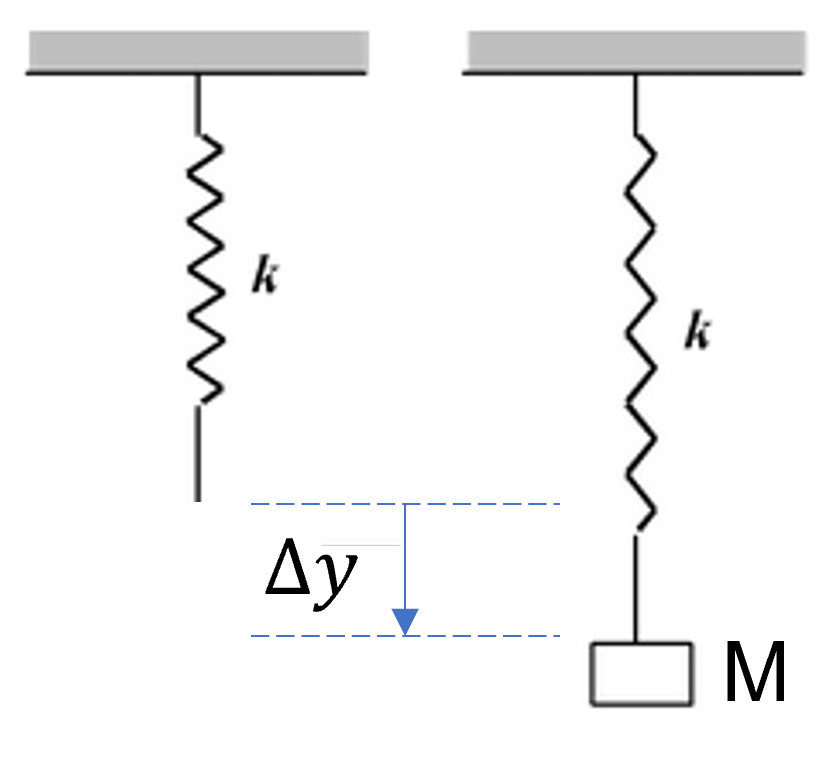
\includegraphics[width=0.35\linewidth]{static.png}
    \caption{Measurement of the elongation of the spring in the static setup.}
    \label{fig:static}
\end{figure}
\subsection*{Measurement}
\begin{itemize}
    \item Use the ruler provided on the setup to measure the displacement of the spring \( \Delta y \) from the photos, see Figure \ref{fig:static}.
    \item Calculate the weight \( W \) of the mass:
    \[
    W = M g
    \]
    where \( g = 9.81 \, \text{m/s}^2 \) is the gravitational acceleration.
    \item Determine the spring constant \( k \) using the formula:
    \[
    k = \frac{W}{\Delta y}
    \]
\end{itemize}
\subsection*{Uncertainty Calculation}
By driving chatGPT with the following prompt or your own modified prompt, determine the mean expected stiffness and it's uncertainty 
\begin{quote}
    \texttt{Propose a method to evaluate the stiffness of a spring by using photos of its initial and deflected states under a static load, with no more than 10 samples from each state, with results including histograms, the mean and standard deviations of deflections, the expected stiffness value and it's uncertainty.}
\end{quote}
Record chatGPT's response, and report it along with the prompt for future reference. If not sure about the meaning of an expected value and it's uncertainty, please ask chatGPT to define them for you. 

\section*{Part 2: Dynamic Method}

\subsection*{Setup}
\begin{itemize}
    \item Use the same spring-mass system.
    \item Attach a different mass \( m = \text{xxx} \, \text{grams} \) to the spring.
\end{itemize}

\subsection*{Procedure}
\begin{enumerate}
    \item Pull the mass down slightly to stretch the spring and then release it to initiate vertical oscillation.
    \item Record the motion of the oscillating mass using a video camera.
\end{enumerate}

\subsection*{Video Analysis}
\begin{itemize}
    \item Use the \textbf{Tracker Video Analysis Tool}: \texttt{https://physlets.org/tracker/}.
    \item Analyze the video to obtain the position-time graph of the mass's vertical motion.
\end{itemize}

\subsection*{Calculation}
\begin{itemize}
    \item Identify the period of the oscillation for the first two complete cycles \( T_1 \) and \( T_2 \), see Figure \ref{fig:dynamic}.
    \begin{figure}
        \centering
        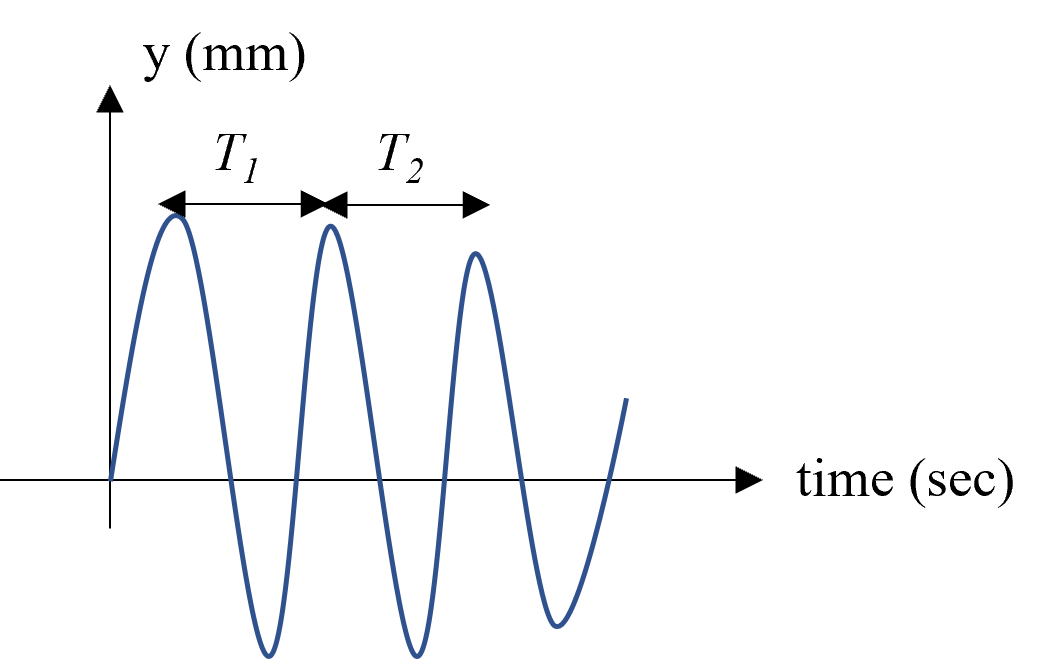
\includegraphics[width=0.5\linewidth]{dynamic.png}
        \caption{Vertical oscillation of the spring-mass system recorded in the dynamic setup}
        \label{fig:dynamic}
    \end{figure}
    \item Use the formula to calculate the spring constant for each period:
    \[
    k = \frac{4\pi^2 m}{T^2}
    \]
    \item Calculate the average \( k_{\text{dynamic}} \) from the two values obtained.
\end{itemize}

\section*{Comparison and Error Analysis}

Compare the static spring constant \( k_{\text{static}} \) with the dynamic spring constant \( k_{\text{dynamic}} \). Use the following formula to calculate the relative error \( E \):
\[
E = \left| \frac{k_{\text{dynamic}} - k_{\text{static}}}{k_{\text{static}}} \right| \times 100
\]
Interpret the results and discuss potential sources of error (e.g., measurement inaccuracies, damping effects, or alignment issues).

\section{Data Analysis}
% --------------------------------------------------------------
\subsection*{1. Equation of Motion of a 1-DOF Spring-Mass System}

A mass $m$ hangs from a spring of stiffness $k$ (N/m). Let $y$ be the position of the mass measured downward from the unstretched spring end. Two vertical forces act on it: the weight $mg$ and the spring force $ky$ (Hooke's law, linear spring). Newton's second law gives
\[
m\ddot y = mg - ky .
\]
At rest ($\ddot y=0$) the mass sits at $y_s = mg/k$, which is the static-method relation $k=mg/\Delta y$ with $\Delta y = y_s$. Measuring from equilibrium, $x = y - y_s$, gives
\[
m\ddot x + kx = 0 .
\]
Gravity has disappeared: it only shifts the equilibrium. A single coordinate $x(t)$ describes the whole system, hence \emph{one degree of freedom}.

\subsubsection{Expert Note:} Real springs also lose energy; adding a viscous force $-c\dot x$ and dividing by $m$,
\[
\ddot x + 2\zeta\omega_n\dot x + \omega_n^2 x = 0,
\qquad \omega_n=\sqrt{k/m},\quad \zeta=\frac{c}{2\sqrt{km}} .
\]
For our spring we expect a small damping ratio $\zeta$; the data will tell us how small.

%--------------------------------------------------------------
\subsection*{2. Dynamic Solution of the Equation of Motion}

For $\zeta=0$, the general solution is $x(t)=A\cos\omega_n t + B\sin\omega_n t$, with $A=x_0$ and $B=v_0/\omega_n$ fixed by the initial position and velocity. Our mass is pulled down and released from rest, so $x(t)=x_0\cos\omega_n t$. The period $T=2\pi/\omega_n=2\pi\sqrt{m/k}$ gives the dynamic-method formula
\[
k=\frac{4\pi^2 m}{T^2}.
\]
$T$ is independent of amplitude and of $g$; heavier masses oscillate more slowly.

\subsubsection{Expert Note:} For light damping ($0<\zeta<1$) the solution is an oscillation inside a decaying envelope,
\[
x(t)=C\,e^{-\zeta\omega_n t}\cos(\omega_d t-\varphi),
\qquad \omega_d=\omega_n\sqrt{1-\zeta^2}.
\]
Inserting the measured damped period $T_d=2\pi/\omega_d$ into $k=4\pi^2m/T^2$ returns $k(1-\zeta^2)$, a relative underestimate of $\zeta^2$. For $\zeta=0.05$ this is only $0.25\,\%$, usually negligible next to other errors.

%--------------------------------------------------------------
\subsection*{3. Determination of Spring Stiffness by the Static Method}

At equilibrium the spring force balances the weight, so
\[
k=\frac{Mg}{\Delta y},\qquad \Delta y=y_f-y_i ,
\]
where $y_i$, $y_f$ are the positions of the same marker (e.g.\ the lower hook) read against the ruler in the two photos. Convert the mass to kilograms. \emph{Example:} $M=200\,\text{g}$, $\Delta y=49\,\text{mm}$ gives $k=0.200\times9.81/0.049\approx 40.0\ \text{N/m}$.

Because $\Delta y$ is a difference, any constant offset (such as the ruler zero) cancels. Keep the camera fixed and perpendicular to the ruler to avoid parallax. A single mass cannot show whether the spring is linear; several masses and a fitted slope of $Mg$ versus $\Delta y$ would average out reading errors and test linearity.

%--------------------------------------------------------------
\subsection*{4. Uncertainty Calculation}

Report a result as a value with an uncertainty, $k=\bar k\pm u_k$. For $n$ repeated readings $y_1,\dots,y_n$ ($n\le10$ per photo):
\[
\bar y=\frac1n\sum_{j}y_j,\qquad
s=\sqrt{\frac{\sum_j(y_j-\bar y)^2}{n-1}},\qquad
u_y=\frac{s}{\sqrt n}.
\]
$s$ is the scatter of single readings and does not shrink with $n$; $u_y$ says how well the mean is known and falls as $1/\sqrt n$. The elongation is a difference of independent means, so $u_{\Delta y}=\sqrt{u_{y_i}^2+u_{y_f}^2}$, and for the quotient $k=Mg/\Delta y$,
\[
\left(\frac{u_k}{k}\right)^2=\left(\frac{u_M}{M}\right)^2+\left(\frac{u_{\Delta y}}{\Delta y}\right)^2 .
\]
In the example, $u_{\Delta y}=0.7\,\text{mm}$ (1.4\,\%) and $u_M=0.1\,\text{g}$ (negligible) give $u_k\approx0.6\ \text{N/m}$, so $k=40.0\pm0.6\ \text{N/m}$. The $\pm$ is one standard uncertainty (about 68\,\% confidence); doubling it gives about 95\,\%. Use these formulas to check ChatGPT's answer, and judge the static--dynamic comparison against the combined uncertainties, not merely by how small the difference looks.

%--------------------------------------------------------------
\subsection*{5. Digitization of Motion Using Tracker}

Tracker extracts object positions from video frames:
\begin{enumerate}
    \item \textbf{Load the clip}, set start/end frames, and check that the frame rate matches the camera setting ($\Delta t=1/\text{fps}$, e.g.\ $33\,\text{ms}$ at 30 fps; slow-motion modes are a common pitfall).
    \item \textbf{Calibrate} with the calibration stick between two ruler marks of known separation.
    \item \textbf{Set the axes}: origin at the equilibrium position, vertical axis along the spring, one consistent sign convention.
    \item \textbf{Mark the mass} in every frame (shift-click or auto-tracker) on a clear feature such as a painted dot.
    \item \textbf{Export} the $t$--$y$ table to a text file or spreadsheet.
\end{enumerate}
Accuracy is limited by pixel size, click precision ($\pm1$--$2$ pixels), motion blur, and a camera that is not level and perpendicular. Note that the oscillation \emph{frequency} depends only on the time base, not on the length calibration, whereas the static method depends directly on the ruler scale.

%--------------------------------------------------------------
\subsection*{6. Curve Fitting to the Time History of Motion}

Rather than reading two periods by eye, we use \emph{all} the digitized points $(t_i, y_i)$ exported by Tracker to a CSV file (one header line, then time in seconds and position in the first two columns). Least squares chooses the parameters $\mathbf p$ of a model $y(t;\mathbf p)$ that minimize
\[
S(\mathbf p)=\sum_i\bigl[y_i-y(t_i;\mathbf p)\bigr]^2 .
\]
For simplicity we fit the undamped solution of Section 2, adding an offset because Tracker's origin is arbitrary and a phase because the clip does not start at a perfect release instant:
\[
y(t)=y_0+A\cos(\omega t+\varphi), \qquad k=m\omega^2 .
\]
The four parameters are $y_0, A, \omega, \varphi$. The fit is done in \texttt{gnuplot}; save the following as \texttt{fit.gp} next to \texttt{data.csv} and run \texttt{gnuplot fit.gp}.
{\footnotesize
\begin{verbatim}
set datafile separator ','
set fit errorvariables              # provides w_err after the fit
m  = 0.250                          # mass in kg
T0 = 0.50                           # rough period read from the graph (s)

stats 'data.csv' every ::1 using 2 nooutput   # skip header line
y0 = STATS_mean                     # initial guesses from the data
A  = (STATS_max - STATS_min)/2
w  = 2*pi/T0
p  = 0.1                            # must be non-zero
f(x) = y0 + A*cos(w*x + p)
fit f(x) 'data.csv' every ::1 using 1:2 via y0, A, w, p

k  = m*w**2
uk = 2*k*w_err/w                    # since k is proportional to w^2
print sprintf("k = %.2f +/- %.2f N/m", k, uk)

set xlabel 't (s)'; set ylabel 'y'
plot 'data.csv' every ::1 using 1:2 title 'data', \
     f(x) title 'fit' lw 2
\end{verbatim}
}
The fit is only as good as its starting values: if it fails or converges to a nonsensical $\omega$, check that \texttt{T0} agrees with the period you see on the Tracker graph. The reported $\omega$ does not depend on the length units of $y$ (metres or millimetres), only on the time column. Afterwards, plot the residuals \texttt{'data.csv' every ::1 using 1:(\$2-f(\$1))}: random scatter about zero is good, while a systematic trend, such as oscillations that shrink with time, means the model is incomplete. The fit uses every sample and is far less sensitive to a single mis-clicked frame than a two-period reading.

\subsection*{Expert Note}

If the residuals show a decaying envelope, fit the damped solution of Section 2 instead. Replace the model and the fit line, and give a small non-zero start value for the decay rate $\sigma=\zeta\omega_n$:
{\footnotesize
\begin{verbatim}
s  = 0.1
f(x) = y0 + A*exp(-s*x)*cos(w*x + p)
fit f(x) 'data.csv' every ::1 using 1:2 via y0, A, s, w, p
k  = m*(w**2 + s**2)          # w is the damped frequency omega_d
\end{verbatim}
}
Because $\omega_d^2+\sigma^2=\omega_n^2$, the stiffness is recovered exactly, whereas the undamped fit returns $m\omega_d^2=k(1-\zeta^2)$, slightly low.

\end{document}

